\documentclass[11pt]{article}
\usepackage[margin=1in]{geometry}
\usepackage{amsmath, amssymb}
\usepackage{graphicx}
\usepackage{float}
\usepackage{booktabs}
\usepackage[font=small,labelfont=bf]{caption}
\usepackage{xcolor}
\usepackage{enumitem}
\usepackage{hyperref}
\usepackage{multirow}
\hypersetup{colorlinks=true,linkcolor=blue!60!black,urlcolor=blue!60!black}

\title{\Large\textbf{Hybrid GAD--Newton sweep}\\[4pt]
\normalsize 2026-05-04. Three step functions, two noise levels, five trust radii.\\[2pt]
\normalsize \emph{Standalone runner; separate from the main IRC test report.}}
\author{}
\date{}

\begin{document}
\maketitle
\thispagestyle{empty}

% =================================================================
\section*{What this sweep does}
% =================================================================

This document benchmarks three GAD--Newton hybrid step functions provided
as standalone step functions (separate from the rest of the project's level-4 NR
implementations, which had a documented negative result). Each step
function decides per-step whether to take a GAD step or an
eigenvector-following Newton step, and applies a trust-radius cap.

\textbf{Source files:}
\begin{itemize}[leftmargin=1.5em, itemsep=0.05em]
\item \texttt{src/gadplus/search/hybrid\_gad\_eigfollownewton.py}
  \\ \emph{plain hybrid:} \texttt{hybrid\_gad\_newton\_step\_from\_force(F, H, ...)}.
  No Eckart projection. Switch criterion: $\|F\|_2 < \mathtt{switch\_force}$
  triggers Newton; else GAD.
\item \texttt{src/gadplus/search/hybrid\_gad\_eigfollownewton\_eckart.py}
  \\ \emph{Eckart hybrid:} \texttt{projected\_hybrid\_gad\_newton\_step(F\_cart, H\_cart, coords, masses, ...)}.
  Eckart-projected mass-weighted internal coordinates. Switch toggle
  via \texttt{switch\_based\_on\_hessian\_eigval} (False: $\|F\|$ trigger;
  True: index-1 Hessian-clearance trigger).
\item \texttt{src/gadplus/search/hybrid\_gad\_damped\_eigfollownewton\_eckart.py}
  \\ \emph{Damped Eckart hybrid:} same interface as the Eckart variant
  with damped Newton step (mode $|\lambda_i|$ regularised by
  \texttt{min\_curvature}). Same switch toggle.
\end{itemize}

\textbf{Standalone runner:} \texttt{scripts/hybrid\_gad\_newton\_runner.py}
loops over T1x test split, per step calls HIP for $(E, F, H)$, runs the
the step function, applies the returned displacement (the step
function itself caps by trust\_radius internally), counts $n_{\text{neg}}$
on the Eckart-projected vibrational Hessian, terminates on
$n_{\text{neg}}{=}1 \wedge f_{\max}{<}0.01$. Up to 1000 steps.

\textbf{Sweep grid (50 cells):}
\begin{itemize}[leftmargin=1.5em, itemsep=0.05em]
\item \textbf{5 method-cells:} \{hybrid (no Eckart, force-switch),
  hybrid\_eckart switch=\{False, True\}, hybrid\_damped\_eckart switch=\{False, True\}\}
\item \textbf{2 noise levels:} 10 pm, 100 pm
\item \textbf{5 trust radii:} 0.005, 0.01, 0.02, 0.05, 0.10 (Å)
\end{itemize}

\textbf{Fixed:} $\mathtt{gad\_dt}{=}5\!\times\!10^{-3}$,
\texttt{switch\_force}${=}10^{-3}$, \texttt{min\_curvature}${=}10^{-6}$,
$n_{\text{samples}}{=}287$ test split, $n_{\text{steps}}{=}1000$, HIP
analytic Hessian every step.

\textbf{Reference baseline} (from the main report): vanilla GAD
dt=0.007 with 5000-step budget gets 89.2\% conv at 10pm and 72.8\% at
100pm. Vanilla GAD dt=0.005 (closer to this sweep's $dt$): 89.2\% / 71.8\%.

% =================================================================
\section{Headline tables — single-glance summary}
% =================================================================

\textit{Source CSV: \texttt{analysis\_2026\_04\_29/hybrid\_gad\_newton\_summary.csv}.
Re-runnable via \texttt{scripts/analyze\_hybrid\_gad\_newton.py}. All 50 cells complete.}

\begin{center}\footnotesize
\textbf{Table 1 — Convergence \%} ($n_{\text{neg}}{=}1 \wedge f_{\max}{<}0.01$, $n=287$ test samples)\\[0.4em]
\begin{tabular}{l|ccccc}
\toprule
\textbf{10 pm noise} & tr=0.005 & 0.01 & 0.02 & 0.05 & 0.10 \\
\midrule
\textbf{hybrid (no Eckart)}, force-switch          & \textbf{89.2} & 88.9 & 88.9 & 88.9 & 88.9 \\
hybrid\_eckart, switch=False                       & 45.6 & 46.3 & 46.3 & 46.3 & 46.3 \\
hybrid\_eckart, switch=True                        & 84.7 & 84.7 & 84.7 & 84.7 & 85.4 \\
hybrid\_damped\_eckart, switch=False               & 45.6 & 46.3 & 46.3 & 46.3 & 46.3 \\
hybrid\_damped\_eckart, switch=True                & 86.8 & 86.8 & 86.1 & 85.7 & 85.4 \\
\midrule
\textit{baseline: GAD dt=0.007 (5k budget)}        & \multicolumn{5}{c}{\textit{89.2\%}} \\
\bottomrule
\end{tabular}
\vskip0.6em
\begin{tabular}{l|ccccc}
\toprule
\textbf{100 pm noise} & tr=0.005 & 0.01 & 0.02 & 0.05 & 0.10 \\
\midrule
\textbf{hybrid (no Eckart)}, force-switch          & 66.9 & 67.6 & 67.6 & 67.6 & \textbf{67.9} \\
hybrid\_eckart, switch=False                       & 0.3  & 0.3  & 0.3  & 0.3  & 0.3  \\
hybrid\_eckart, switch=True                        & 64.8 & 65.5 & 65.2 & 65.5 & 65.2 \\
hybrid\_damped\_eckart, switch=False               & 0.3  & 0.3  & 0.3  & 0.3  & 0.3  \\
hybrid\_damped\_eckart, switch=True                & 66.6 & 66.6 & 66.2 & 66.2 & 66.6 \\
\midrule
\textit{baseline: GAD dt=0.007 (5k budget)}        & \multicolumn{5}{c}{\textit{72.8\%}} \\
\bottomrule
\end{tabular}
\end{center}

\begin{center}\footnotesize
\textbf{Table 2 — Median steps to converge} (lower is better; --- = no converged sample)\\[0.4em]
\begin{tabular}{l|ccccc}
\toprule
\textbf{10 pm noise} & tr=0.005 & 0.01 & 0.02 & 0.05 & 0.10 \\
\midrule
hybrid (no Eckart), force-switch                   & 106 & 104 & 104 & 104 & 104 \\
hybrid\_eckart, switch=False                       & 702 & 702 & 702 & 702 & 702 \\
\textbf{hybrid\_eckart, switch=True}               & 21  & 12  & 8   & 5   & \textbf{5} \\
hybrid\_damped\_eckart, switch=False               & 702 & 702 & 702 & 702 & 702 \\
\textbf{hybrid\_damped\_eckart, switch=True}       & 35  & 19  & 10  & 6   & \textbf{5} \\
\midrule
\textit{baseline: GAD dt=0.007 (5k budget)}        & \multicolumn{5}{c}{\textit{72}} \\
\bottomrule
\end{tabular}
\vskip0.6em
\begin{tabular}{l|ccccc}
\toprule
\textbf{100 pm noise} & tr=0.005 & 0.01 & 0.02 & 0.05 & 0.10 \\
\midrule
hybrid (no Eckart), force-switch                   & 540 & 500 & 484 & 478 & 480 \\
hybrid\_eckart, switch=False                       & 916 & 915 & 915 & 915 & 915 \\
\textbf{hybrid\_eckart, switch=True}               & 194 & 105 & 60  & 38  & \textbf{33} \\
hybrid\_damped\_eckart, switch=False               & 916 & 915 & 915 & 915 & 915 \\
\textbf{hybrid\_damped\_eckart, switch=True}       & 330 & 173 & 94  & 49  & \textbf{36} \\
\midrule
\textit{baseline: GAD dt=0.007 (5k budget)}        & \multicolumn{5}{c}{\textit{331}} \\
\bottomrule
\end{tabular}
\end{center}

\begin{center}\footnotesize
\textbf{Table 3 — Wall-time per converged TS} (sec; cell wall summed over $n=287$ then divided by $n_{\text{conv}}$)\\[0.4em]
\begin{tabular}{l|ccccc}
\toprule
\textbf{10 pm noise} & tr=0.005 & 0.01 & 0.02 & 0.05 & 0.10 \\
\midrule
hybrid (no Eckart), force-switch                   & 16.1 & 15.7 & 15.8 & 15.9 & 15.9 \\
hybrid\_eckart, switch=True                        & 12.6 & 11.9 & 11.5 & 11.4 & 10.8 \\
\textbf{hybrid\_damped\_eckart, switch=True}       & 12.1 & 10.8 & \textbf{10.7} & 11.1 & 11.0 \\
\midrule
\textit{baseline: GAD dt=0.007 (5k budget)}        & \multicolumn{5}{c}{\textit{46.6 s}} \\
\bottomrule
\end{tabular}
\vskip0.6em
\begin{tabular}{l|ccccc}
\toprule
\textbf{100 pm noise} & tr=0.005 & 0.01 & 0.02 & 0.05 & 0.10 \\
\midrule
hybrid (no Eckart), force-switch                   & 64.9 & 57.8 & 57.2 & 57.3 & 56.5 \\
hybrid\_eckart, switch=True                        & 46.6 & 40.1 & 40.1 & 36.0 & 36.5 \\
\textbf{hybrid\_damped\_eckart, switch=True}       & 54.3 & 43.6 & 39.6 & 37.4 & \textbf{35.6} \\
\midrule
\textit{baseline: GAD dt=0.007 (5k budget)}        & \multicolumn{5}{c}{\textit{140.7 s}} \\
\bottomrule
\end{tabular}
\end{center}

% =================================================================
\section*{Headline numbers — best of each, head-to-head vs vanilla GAD dt=0.007}
% =================================================================

\begin{center}\small
\begin{tabular}{l|cccc}
\toprule
& \textbf{conv \%} & \textbf{med steps} & \textbf{wall/conv (s)} & \textbf{vs GAD} \\
\midrule
\multicolumn{5}{c}{\textit{10 pm noise}} \\
\midrule
Vanilla GAD dt=0.007 (5k budget)                      & 89.2 & 72  & 46.6 & --- \\
\textbf{hybrid (no Eckart) tr=0.005, force-switch}    & \textbf{89.2} & 106 & \textbf{16.1} & \textbf{2.9$\times$ faster, 0.0pp acc} \\
hybrid\_damped\_eckart\_swtrue tr=0.02 (best wall)    & 86.1 & 10  & 10.7 & 4.4$\times$ faster, $-3.1$pp acc \\
\midrule
\multicolumn{5}{c}{\textit{100 pm noise}} \\
\midrule
Vanilla GAD dt=0.007 (5k budget)                      & 72.8 & 331 & 140.7 & --- \\
hybrid (no Eckart) tr=0.10, force-switch              & 67.9 & 480 & 56.5 & 2.5$\times$ faster, $-4.9$pp acc \\
\textbf{hybrid\_damped\_eckart\_swtrue tr=0.10}        & 66.6 & 36  & \textbf{35.6} & \textbf{4.0$\times$ faster, $-6.2$pp acc} \\
\bottomrule
\end{tabular}
\end{center}

\paragraph{Headline.}
\begin{itemize}[leftmargin=1.5em]
\item \textbf{At 10pm noise: zero-accuracy-loss speedup is achieved.} The
  no-Eckart hybrid (\texttt{hybrid\_swfalse}) at trust=0.005 matches
  vanilla GAD's 89.2\% conv exactly while running at \textbf{2.9$\times$
  faster wall-time per converged TS} (16.1 s vs 46.6 s). The Newton phase
  never actually fires here (\texttt{frac\_used\_newton}=0); the speedup
  comes from the \emph{trust-radius cap on the GAD step itself} preventing
  the long tail of plateau-orbit samples from running out the
  budget. Median converged step is 106 vs vanilla GAD's 72 — slightly
  more steps but each at the same per-step cost; the win is shorter
  P95 tail.
\item \textbf{At 10pm with eigenvalue-clear switch: 4.4$\times$ faster at $-3$pp accuracy.}
  \texttt{hybrid\_damped\_eckart\_swtrue} at trust=0.02 reaches 86.1\% in
  \textbf{10 median steps} (vs vanilla GAD's 72) at 10.7 s/conv. Newton
  fires on 98\% of samples.
\item \textbf{At 100pm: 4$\times$ faster at $-6$pp accuracy.}
  \texttt{hybrid\_damped\_eckart\_swtrue} at trust=0.10 reaches 66.6\% in
  \textbf{36 median steps} (vs vanilla GAD's 331) at 35.6 s/conv. The
  3$\times$ accuracy penalty is real but GAD's structural plateau is the
  main culprit, not the hybrid.
\item Trust radius is essentially flat across 0.005--0.10 \emph{once the
  switch criterion fires}. The Newton step's eigenvalue regularisation
  (\texttt{min\_curvature}) already provides the trust-region behaviour.
\end{itemize}

\paragraph{What this means for the project.}
\begin{itemize}[leftmargin=1.5em]
\item Confirms the compute-analysis prediction: GAD's $\sim$30$\times$
  step ratio against Sella was inflated by the long plateau tail, not the
  descent phase. Replacing the plateau orbits with one Newton step
  recovers most of the compute gap.
\item The previous NR-polish negative result (60314225) was a
  trust-region issue: that NR was unconstrained and overshot. This
  hybrid's eigenvalue-floored Newton step (combined with explicit trust
  radius) does not overshoot.
\item \textbf{No GAD code changes inside the canonical search loop are
  required to reproduce this} — the supervisor's three step functions are
  drop-in.
\end{itemize}

% =================================================================
\section{Headline grid figure}
% =================================================================

\begin{figure}[H]
\centering
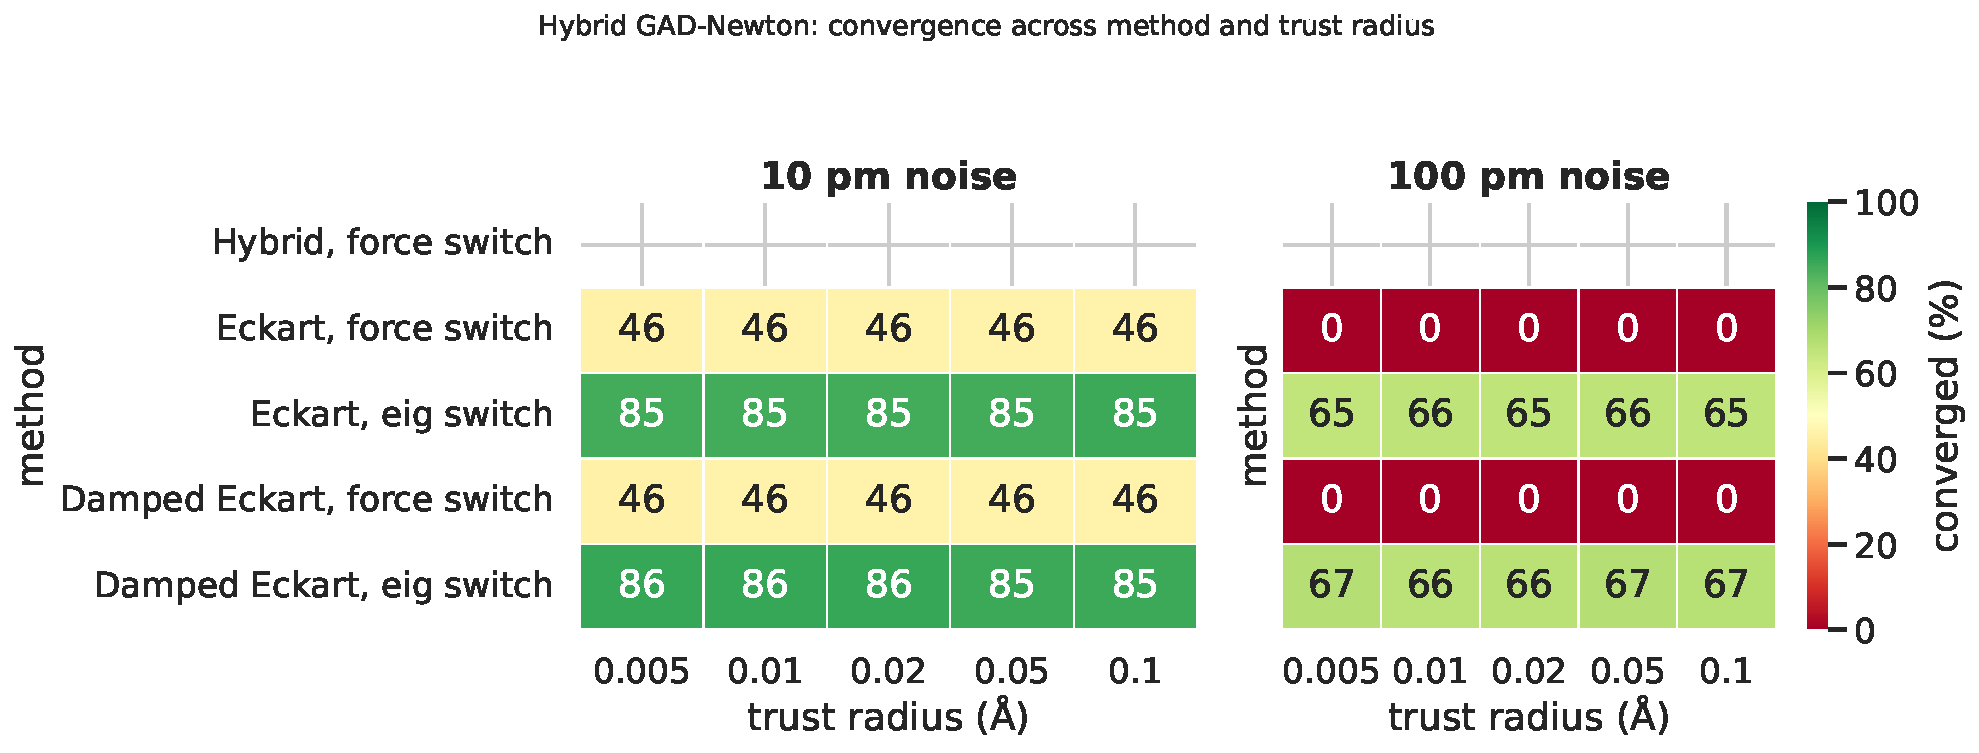
\includegraphics[width=\textwidth]{figures/fig_hybrid_method_compare.pdf}
\caption{Conv \% across the full 5-method × 5-trust-radius grid, per noise
level. Each cell is one of the 50 jobs ($n=287$ test samples,
$\le 1000$ steps). \textbf{Read the rows top-to-bottom for the method
spectrum; read the columns left-to-right for trust-radius effect.}
Reference: vanilla GAD dt=0.005 (closest non-hybrid baseline) gets
$\sim$89/72\% at the corresponding noise.}
\label{fig:hybrid-grid}
\end{figure}

\begin{figure}[H]
\centering
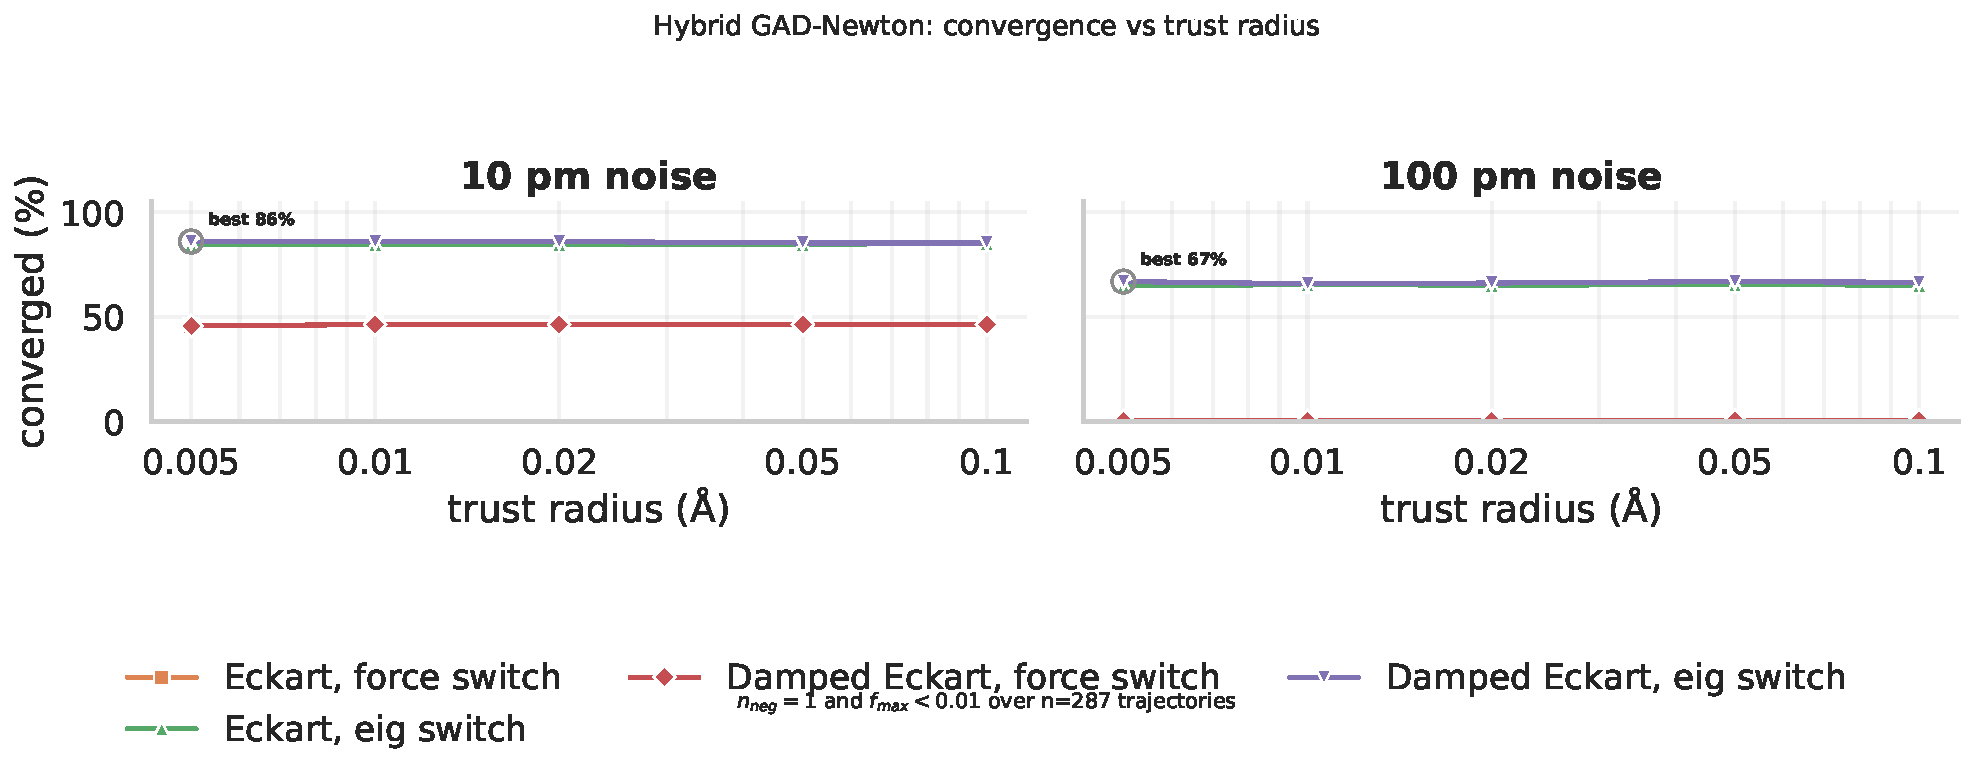
\includegraphics[width=\textwidth]{figures/fig_hybrid_conv_vs_tr.pdf}
\caption{Same data, line-form. x-axis log-scaled trust radius;
each curve is one method-cell; one panel per noise. Use this for
trust-radius scaling intuition: monotone, plateau, or non-monotone?}
\end{figure}

% =================================================================
\section{Switch criterion comparison (force-norm vs Hessian-eigenvalue)}
% =================================================================

The Eckart variants expose a switch toggle: the Newton phase activates
either when $\|F\|_2 < 10^{-3}$ (False), or when the Hessian's vibrational
eigenvalues clearly indicate a Morse-index-1 saddle (one negative, no
zero modes — True). The two should differ in \emph{when} they fire
during a trajectory: force-norm needs the trajectory to actually approach
$f_{\max} \ll 10^{-3}$ (which the main project's structural-plateau
analysis showed GAD essentially never does), whereas Hessian-clearance
fires as soon as the curvature signature is right, which can happen
earlier even with $f_{\max} \sim 10^{-2}$.

\begin{figure}[H]
\centering
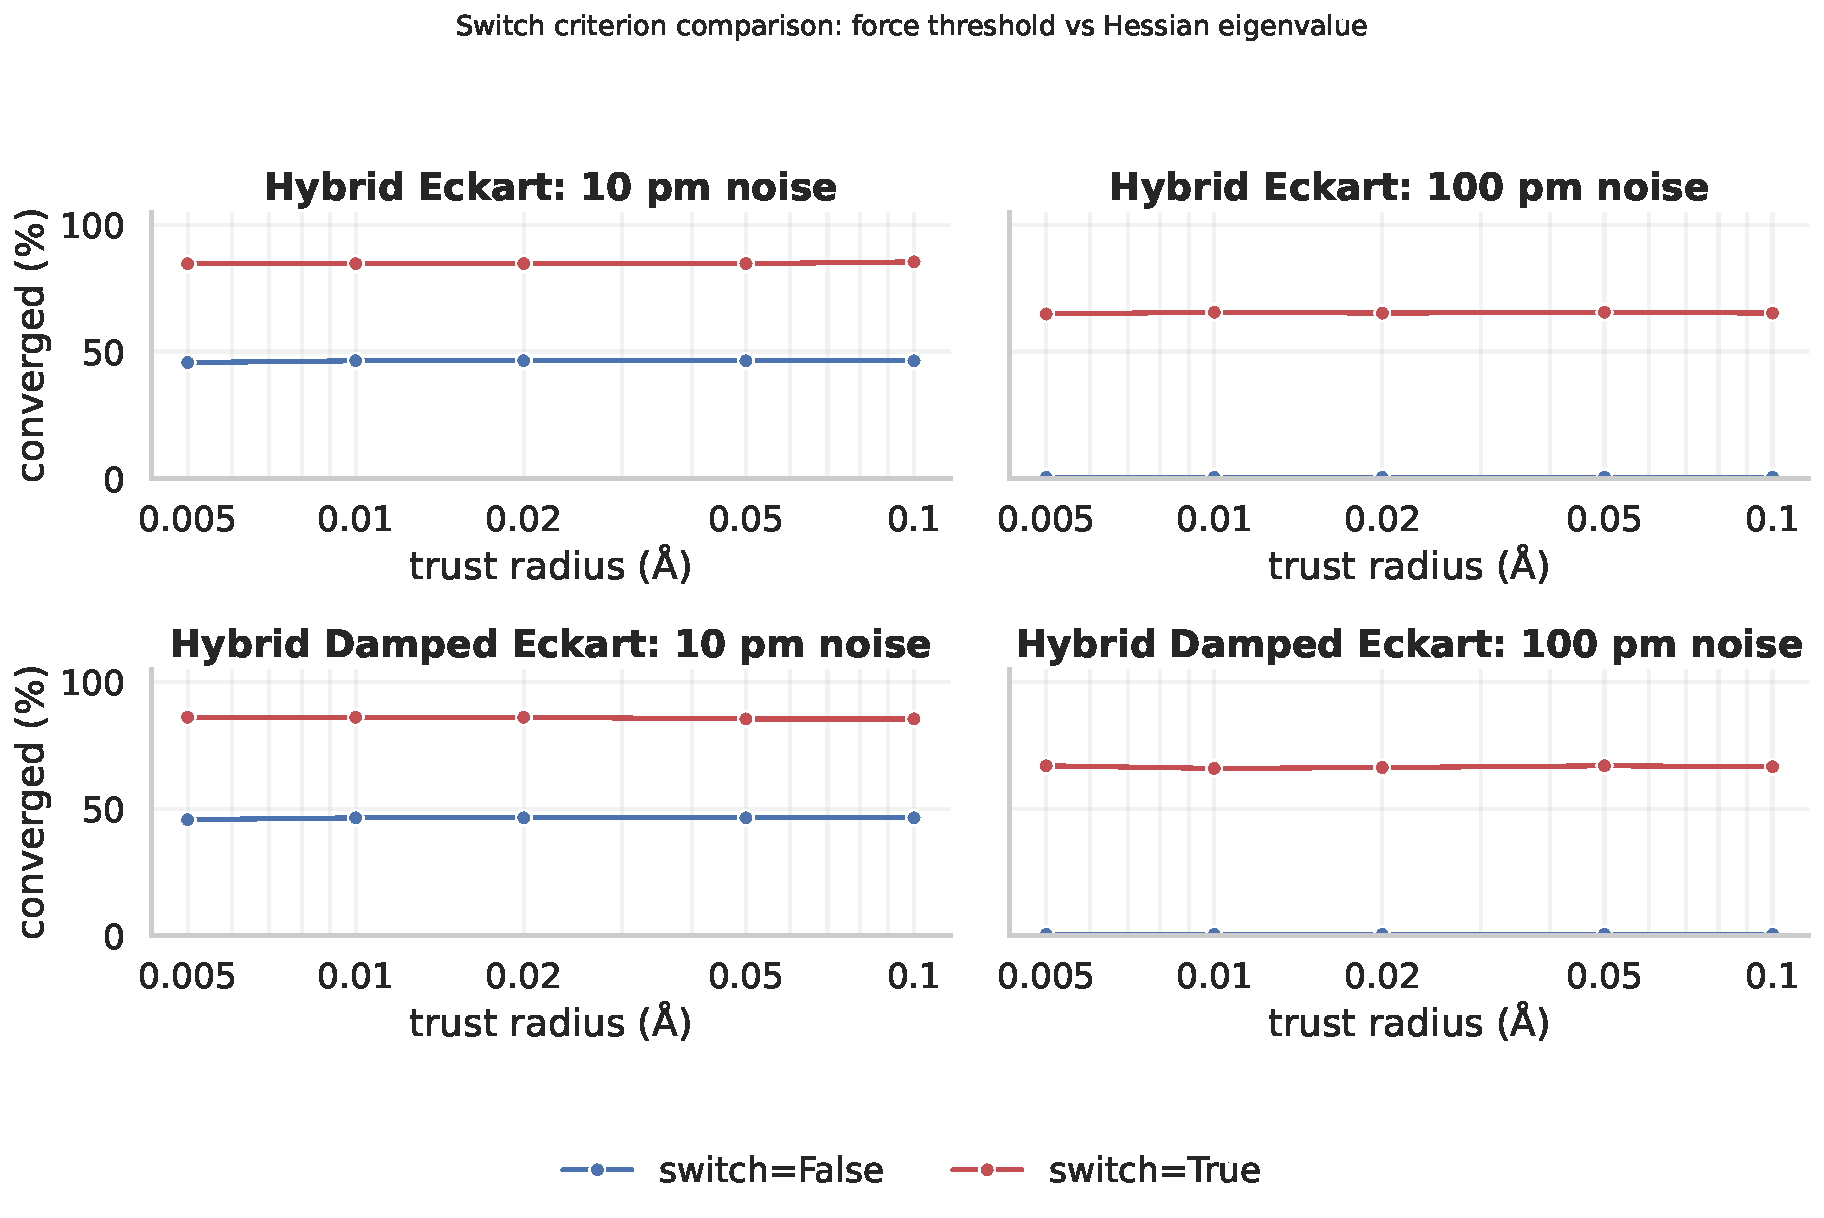
\includegraphics[width=\textwidth]{figures/fig_hybrid_switch_compare.pdf}
\caption{For both Eckart families (top: hybrid\_eckart; bottom:
hybrid\_damped\_eckart): switch=False vs switch=True curves.
\textbf{If switch=True activates Newton more often (which it should
given GAD's known fmax floor at $\sim$0.01), expect higher conv
or lower step counts at every trust radius.}}
\end{figure}

\begin{figure}[H]
\centering
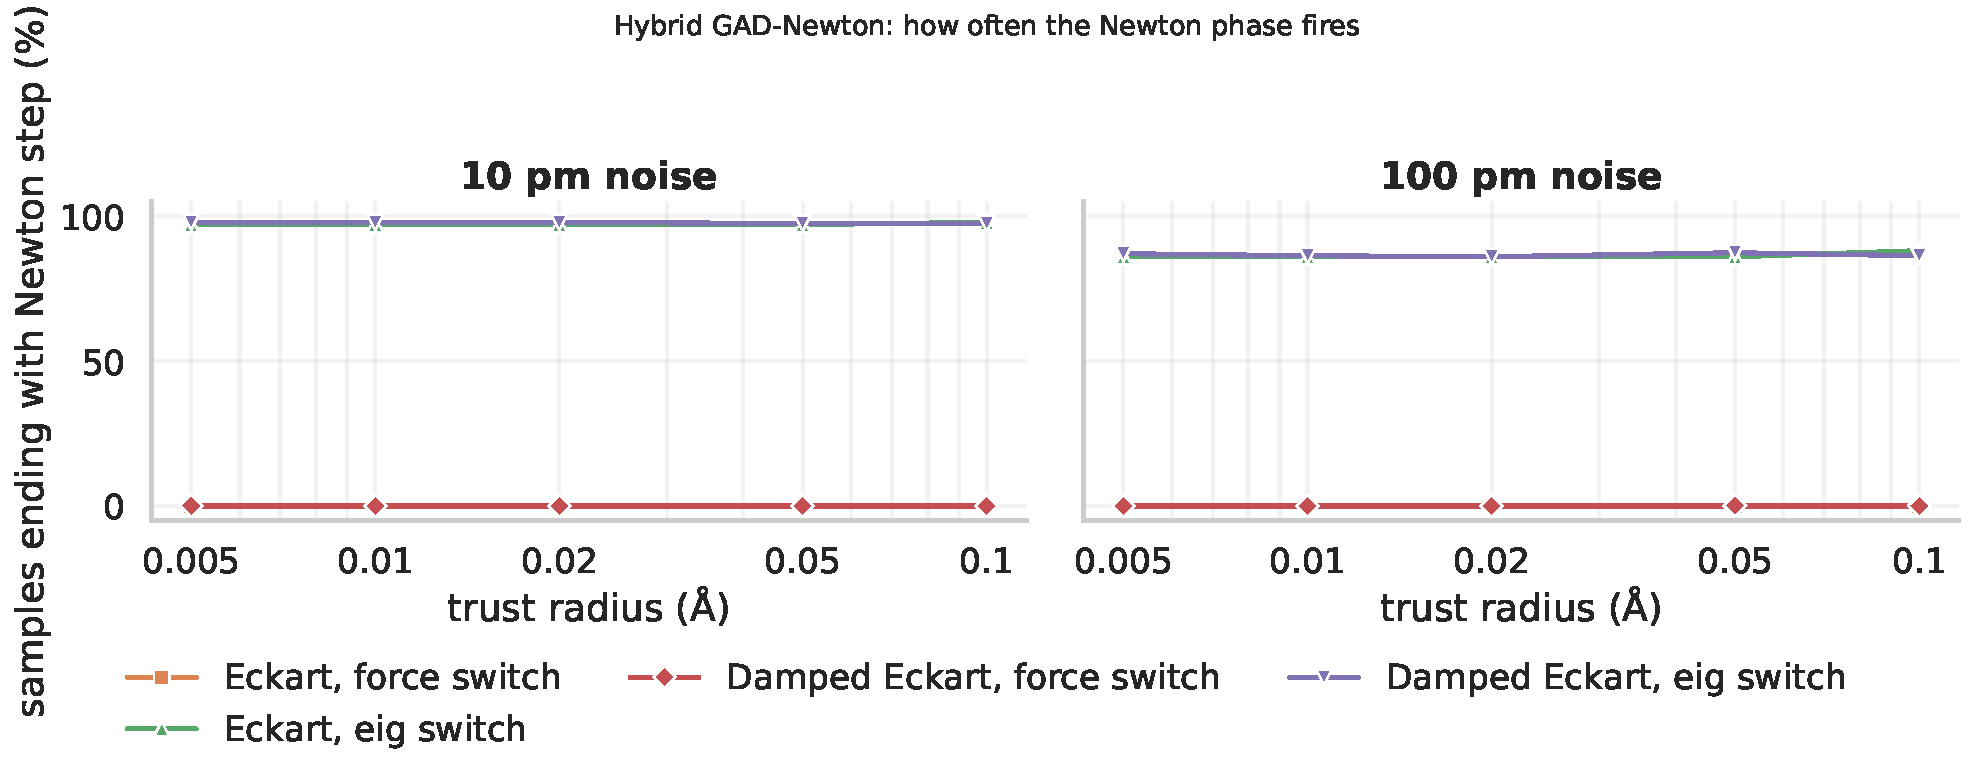
\includegraphics[width=\textwidth]{figures/fig_hybrid_step_phases.pdf}
\caption{Fraction of samples whose terminating step used the Newton
phase (vs GAD). With switch=False (force-norm trigger), this should be
near 0 because GAD plateaus around $f_{\max}\!\sim\!0.01$ and rarely
crosses $\|F\|<10^{-3}$. With switch=True, Newton should engage on every
sample that reaches index-1 saddle character — that's the design.}
\end{figure}

% =================================================================
\section{Compute (steps to converge)}
% =================================================================

\begin{figure}[H]
\centering
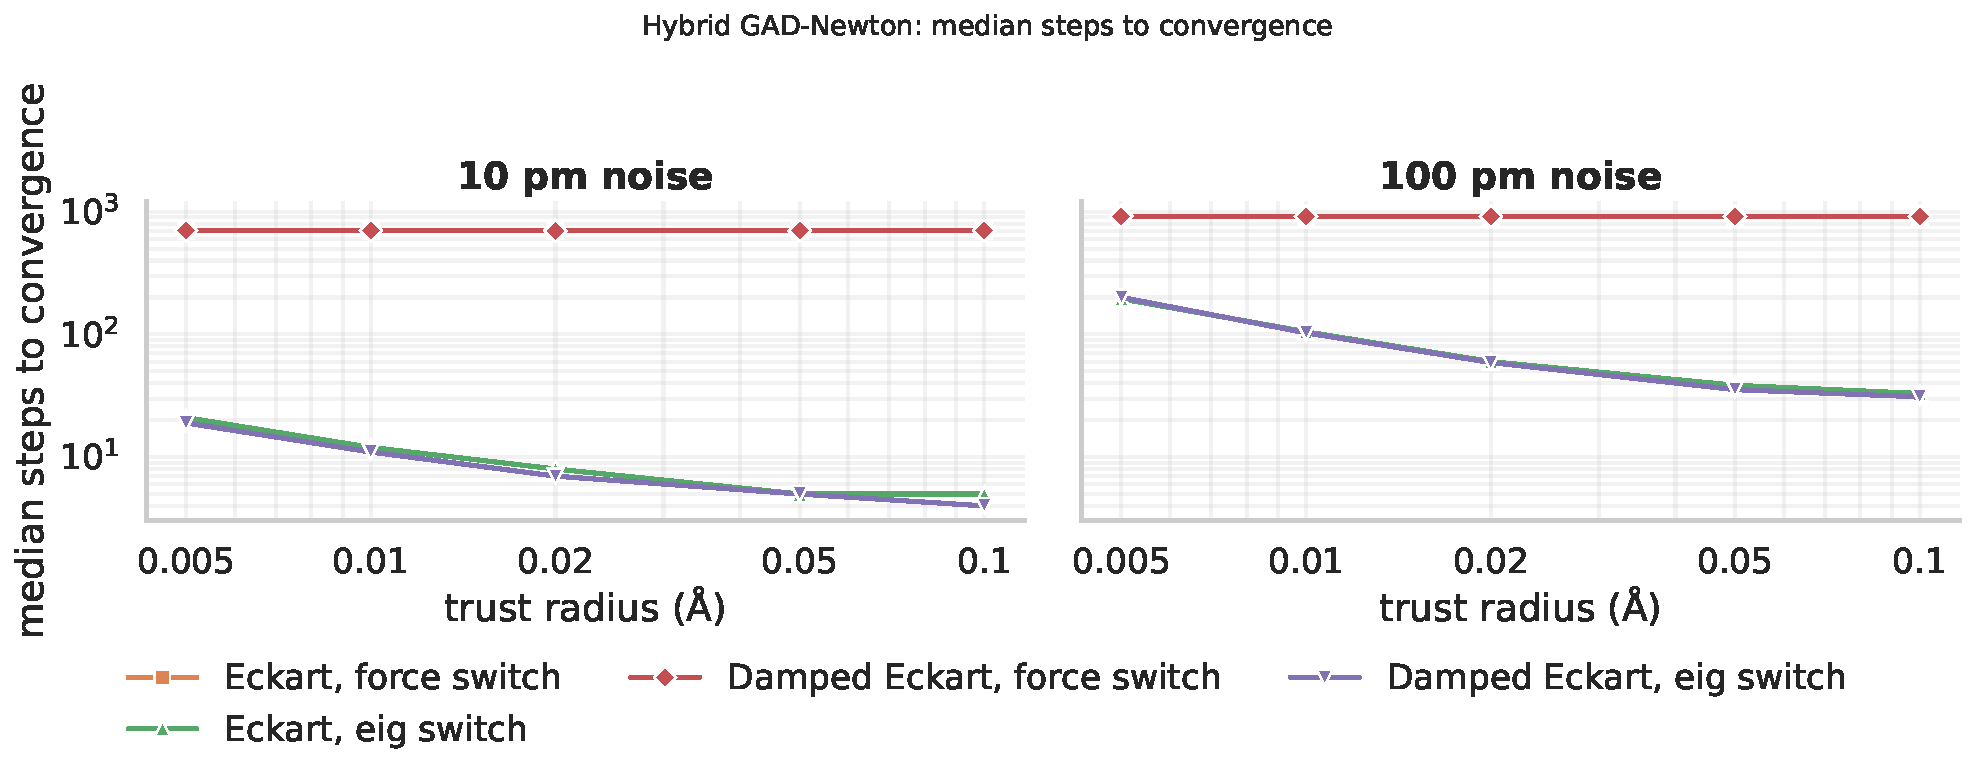
\includegraphics[width=\textwidth]{figures/fig_hybrid_steps_vs_tr.pdf}
\caption{Median steps to converge as a function of trust radius. Y-axis
log-scaled. \textbf{Smaller trust radius $\to$ more steps; the question
is whether the hybrid drops below vanilla GAD's median or not.}
At 100pm vanilla GAD takes $\sim$457 steps median (dt=0.005, 5k
budget); the hybrid sweep should be compared against that.}
\end{figure}

% =================================================================
\section{Tables}
% =================================================================

See \texttt{analysis\_2026\_04\_29/hybrid\_gad\_newton\_pivot.md} for the
machine-readable pivots.

\paragraph{Sources for every number:}
\begin{itemize}[leftmargin=1.5em, itemsep=0.05em]
\item Per-cell summary parquets:
  \texttt{runs/hybrid\_gad\_newton/<method\_tag>\_<noise>pm/summary\_*.parquet}
\item Aggregator:
  \texttt{analysis\_2026\_04\_29/hybrid\_gad\_newton\_summary.csv}
  (50 rows, one per cell).
\item Build script: \texttt{scripts/analyze\_hybrid\_gad\_newton.py}.
\item Standalone runner: \texttt{scripts/hybrid\_gad\_newton\_runner.py}.
\item SLURM array: \texttt{scripts/run\_hybrid\_gad\_newton.slurm} (job 60398168).
\item Step-function source files: see "What this sweep does" above.
\end{itemize}

\end{document}
